\documentclass[12pt]{article}

\usepackage[margin=1in]{geometry}
\usepackage{amsmath,amsthm,amssymb}
\usepackage{fancyhdr}
\usepackage[small,compact]{titlesec}
\usepackage{float}

\lhead{Erich Menge}
\chead{\classnameandsection}
\rhead{\homeworktitle}

\pagestyle{fancy}

\newcommand{\sethomeworknumber}[1]{
  \newcommand{\homeworktitle}{Homework #1}
}

\newcommand{\N}{\mathbb{N}}
\newcommand{\Z}{\mathbb{Z}}
\newcommand{\homeworkheader}[1]{
  \title{\vspace{2in}\homeworktitle}
  \author{Erich Menge (X.500: menge053, Student ID: 4624713) \\
  #1}
  \maketitle
  \newpage
}

\newenvironment{problem}[1]{
  \ignorespaces
  \section*{Problem #1}
}{
  \ignorespacesafterend
}

\newenvironment{solution}{
  \ignorespaces
  \subsection*{Solution}
}{
  \ignorespacesafterend
}

\newcommand{\classnameandsection}{CSCI 4011 Formal Languages And Automata Theory Section 3}

\usepackage{subfigure}
\usepackage{graphicx}

\sethomeworknumber{3}

\begin{document}
\homeworkheader{\classnameandsection}

\begin{problem}{1}
  1a. $\{w \in \{a,b\}^*\ |\ \text{w has twice as many bs as as} \}$
  \br
  1b. Balanced parentheses and square brackets. Thus, ()(), [][] and (([])[()]) would be legal expressions of this
     language but ([)] and [(()] would not.
  \br
  1c. The language in Exercise 2.6, part d, in the book.
  \br
  1d. $\{ a^ib^jc^k | i = j or j = k \}$
  \br
  2. We will observe (without proof) in class that any grammar for the language in part (d) above must be ambiguous.
     Exhibit this ambiguity for the grammar you have provided by showing two different parse trees for a suitably chosen
     string in the language.
  \begin{solution}
    1a. At first I was tempted to do something like $S \rightarrow bab | bba | abb | A | \epsilon$ but that wouldn't
    allow for long chains such as $aabaabbbbbbb$. \\ So instead it should be $S \rightarrow bSaSb | bSbSa |
    aSbSb|\epsilon$. Which is much like above except it separates each character with $S$ to allow enough flexibility
    for the $\Sigma^*$ requirement.
    \br
    1b. $S \rightarrow (S)\ |\ [S]\ |\ \epsilon$
    \br
    1c.
    \br
    1d.
    \begin{align*}
      S &\rightarrow BC'|AC \\
      B &\rightarrow aBb | \epsilon \\
      C &\rightarrow bCc | \epsilon \\
      C' &\rightarrow cC' | \epsilon \\
      A &\rightarrow aA | \epsilon
    \end{align*}
    So this says from our start position we can have balanced $a$s and $b$s followed by any number of $c$s, or we can
    have any number of $a$s followed by balanced $b$s and $c$s.
    \br
    2. If we select a string which belongs to both, such as $abc$, we can get two parse trees.
    \begin{figure}[H]
      \centering
      \caption{Two Parse Trees for the Same CFG}
      \subfigure[Tree 1]{
        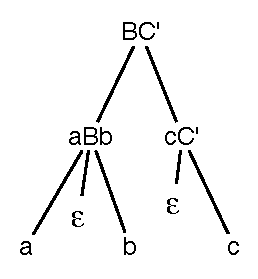
\includegraphics{problem_1_2_a.eps}
      }
      \subfigure[Tree 2]{
        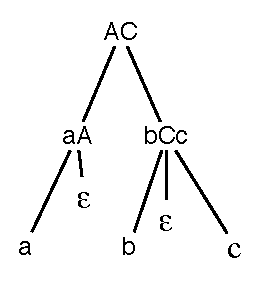
\includegraphics{problem_1_2_b.eps}
      }
    \end{figure}
  \end{solution}
\end{problem}

\begin{problem}{2}
\end{problem}

\begin{problem}{3}
  \begin{solution}
    We have a 6 tuple $<Q, \Sigma, \Gamma, \delta, q_1, F>$ \\
    \(
      Q = \{ q_1, q_2, \ldots, q_{11} \} \\
      \Sigma = \{ a, b \} \\
      \Gamma = \{R, S, T, X \} \cup \Sigma \\
      F = \{ Q_{11} \}
    \) \\
    And $\delta$ the transition function is represented by the figure below.
    \begin{figure}[H]
      \centering
      \caption{Transitions for PDF recognizing the grammar}
      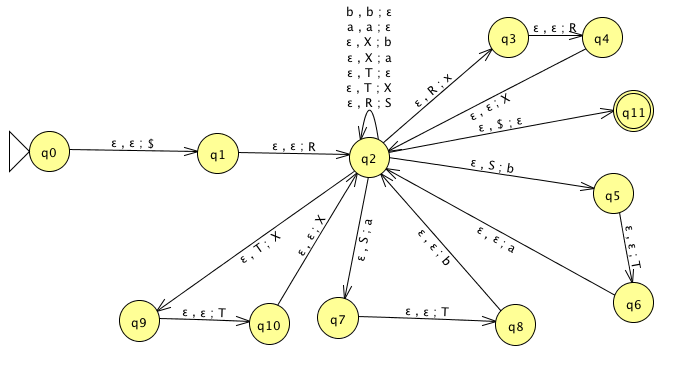
\includegraphics[scale=.6]{problem_2.png}
    \end{figure}
  \end{solution}
\end{problem}

\begin{problem}{4}
\end{problem}

\begin{problem}{5}
\end{problem}

\begin{problem}{6}
\end{problem}

\begin{problem}{7}
\end{problem}

\begin{problem}{8}
\end{problem}

\begin{problem}{9}
\end{problem}



\end{document}
